\chapter{Automated Distribution of Quantum Algorithms}
\label{chap:Project}

\section{Implementing non-local CNOT gates}
\label{NonLocalGates}

In \S\ref{IntroDistributing}, we explained the proposal by~\citet{NonLocalCNOT} of how to implement a non-local gate. We will now extend their results.

In the original work, in order to implement multiple non-local gates using a single ebit, there must not be any operation on the control qubit between the non-local gates. However, many of the 1-qubit gates from the Clifford+T set commute with the CNOT gate. This means that, if there are operations in between CNOTs, we may transform the circuit to an equivalent version where the CNOT gates are brought together. And although some of the gates do not commute with CNOT, in some cases they can still be interchanged with it if an additional 1-qubit gate is added. All of the relevant circuit transformations are shown in Figure~\ref{fig:pullRules}. These can be checked by calculating the corresponding matrices of both sides and verifying they match.

\begin{figure}
\hspace*{-6mm}
\begin{tikzpicture}
  \node[font=\itshape] (textA) {\(\forall g\in\{Z,S,T\}\) at control wire};
  \node [below=-5mm of textA] (A) {
    \begin{tikzpicture}
      \node[inner sep=0pt] (c1) at (0,0) {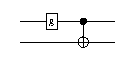
\includegraphics[scale=2]{Figures/circuits/C_gCNOT}};       
      \node[right=-13.9mm of c1.east, inner sep=0pt] (c2) {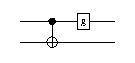
\includegraphics[scale=2]{Figures/circuits/C_CNOTg}};
      \node[right=-12mm of c1.east, rectangle, fill=white, minimum size=10mm] (eq) {\(=\)};  
      \node[right=7mm of c1.west, rectangle,fill=white,minimum width=5mm, minimum height=10mm] {};
      \node[left=7mm of c2.east, rectangle,fill=white,minimum width=5mm, minimum height=10mm] {};
    \end{tikzpicture}
  };
  \node[right=20mm of textA, font=\itshape] (textB) {\(\forall g\!\text{'}\in\{X,Y\}\) at control wire};
  \node [below=-5mm of textB] (B) {
    \begin{tikzpicture}
      \node[inner sep=0pt] (c1) at (0,0) {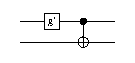
\includegraphics[scale=2]{Figures/circuits/C_g2CNOT}};       
      \node[right=-13.9mm of c1.east, inner sep=0pt] (c2) {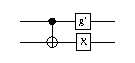
\includegraphics[scale=2]{Figures/circuits/C_CNOTg2}};
      \node[right=-12mm of c1.east, rectangle, fill=white, minimum size=10mm] (eq) {\(=\)};  
      \node[right=7mm of c1.west, rectangle,fill=white,minimum width=5mm, minimum height=10mm] {};
      \node[left=7mm of c2.east, rectangle,fill=white,minimum width=5mm, minimum height=10mm] {};
    \end{tikzpicture}
  };
  \node[below=20mm of textA, font=\itshape] (textC) {\(\forall g\in\{X\}\) at target wire};
  \node [below=-5mm of textC] (C) {
    \begin{tikzpicture}
      \node[inner sep=0pt] (c1) at (0,0) {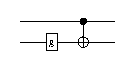
\includegraphics[scale=2]{Figures/circuits/T_gCNOT}};       
      \node[right=-13.9mm of c1.east, inner sep=0pt] (c2) {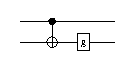
\includegraphics[scale=2]{Figures/circuits/T_CNOTg}};
      \node[right=-12mm of c1.east, rectangle, fill=white, minimum size=10mm] (eq) {\(=\)};  
      \node[right=7mm of c1.west, rectangle,fill=white,minimum width=5mm, minimum height=10mm] {};
      \node[left=7mm of c2.east, rectangle,fill=white,minimum width=5mm, minimum height=10mm] {};
    \end{tikzpicture}
  };
  \node[below=20mm of textB, font=\itshape] (textD) {\(\forall g\!\text{'}\in\{Y,Z\}\) at target wire};
  \node [below=-5mm of textD] (D) {
    \begin{tikzpicture}
      \node[inner sep=0pt] (c1) at (0,0) {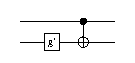
\includegraphics[scale=2]{Figures/circuits/T_g2CNOT}};       
      \node[right=-13.9mm of c1.east, inner sep=0pt] (c2) {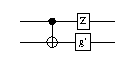
\includegraphics[scale=2]{Figures/circuits/T_CNOTg2}};
      \node[right=-12mm of c1.east, rectangle, fill=white, minimum size=10mm] (eq) {\(=\)};  
      \node[right=7mm of c1.west, rectangle,fill=white,minimum width=5mm, minimum height=10mm] {};
      \node[left=7mm of c2.east, rectangle,fill=white,minimum width=5mm, minimum height=10mm] {};
    \end{tikzpicture}
  };
\end{tikzpicture}
\caption{Different cases when a 1-qubit gate from Clifford+$T$ can be pushed through a CNOT gate.}
\label{fig:pullRules}
\end{figure}

The second improvement comes by realising that the method used to implement multiple CNOT gates controlled by the same wire (explained in \S\ref{IntroDistributing}) can also be applied if multiple CNOT have a common target qubit instead. We will refer to the former method as the \textit{common-control} method and \textit{common-target} for the latter. The derivation of the common-target method is shown in Figure~\ref{fig:CNOTtargetProof}, which uses some of the properties listed in \S\ref{Models}. The main difference is that the CNOT itself is now applied in the control QPU instead of the target, so the cat-entangler and cat-disentangler must change accordingly.

\begin{figure}
\vspace*{11mm}
\hspace*{73mm}
\begin{tikzpicture}[transform canvas={scale=0.73}]
  \node (A) {
    \begin{tikzpicture}
      \node[inner sep=0pt] (c1) {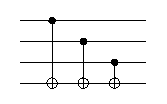
\includegraphics[scale=2]{Figures/circuits/proof1}};  
      \coordinate[below left=7mm and -6mm of c1.west] (l1);
      \coordinate[right=45mm of l1] (r1);
      \pic (cut1) {cut=l1/r1};     
      \node[right=0mm of c1] (eq1) {\Large \(=\)}; 
      \node[right=0mm of eq1, inner sep=0pt] (c2) {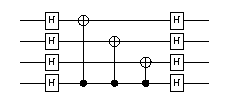
\includegraphics[scale=2]{Figures/circuits/proof2}};  
      \coordinate[below left=7mm and -6mm of c2.west] (l2);
      \coordinate[right=66mm of l2] (r2);
      \pic (cut2) {cut=l2/r2};  
      \node[right=0mm of c2] (eq2) {\Large \(=\)};  
    \end{tikzpicture}
  };
  \node[below=5mm of A] (B) {
    \begin{tikzpicture}
      \node (eq2) {\Large \(=\)};    
      \node[right=-4mm of eq2, inner sep=0pt] (circuit) {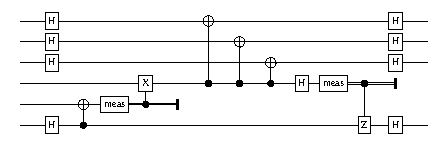
\includegraphics[scale=2]{Figures/circuits/proof3}};  
      \pic (e3) {ebit=e3/26.79mm/13mm};  
      \coordinate[below left=7mm and -6mm of circuit.west] (l3);
      \coordinate[right=140mm of l3] (r3);
      \pic (cut3) {cut=l3/r3};  
      \node[right=0mm of circuit] (eq3) {\Large \(=\)}; 
    \end{tikzpicture}
  };
  \node[below=5mm of B] (C) {
    \begin{tikzpicture}
      \node (eq3) {\Large \(=\)}; 
      \node[right=0mm of eq3, inner sep=0pt] (circuit) {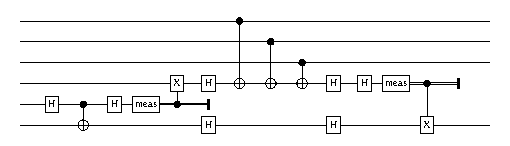
\includegraphics[scale=2]{Figures/circuits/proof4}};   
      \pic (e4) {ebit=e4/26.79mm/13mm};  
      \coordinate[below left=7mm and -6mm of circuit.west] (l4);
      \coordinate[right=161mm of l4] (r4);
      \pic (cut4) {cut=l4/r4};  
      \node[right=0mm of circuit] (eq4) {\Large \(=\)}; 
    \end{tikzpicture}
  };
  \node[below=5mm of C] (D) {
    \begin{tikzpicture}
      \node (eq4) {\Large \(=\)};    
      \node[right=-4mm of eq4, inner sep=0pt] (circuit) {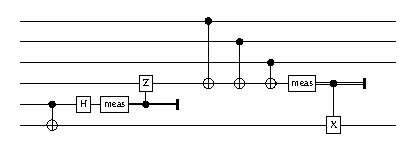
\includegraphics[scale=2]{Figures/circuits/proof5}};     
      \pic (e5) {ebit=e5/26.79mm/13mm};  
      \coordinate[below left=7mm and -6mm of circuit.west] (l5);
      \coordinate[right=129mm of l5] (r5);
      \pic (cut5) {cut=l5/r5};  
      \node[right=-4mm of circuit] (eq5) {\Large \(=\)};    
      \node[right=-4mm of eq5, inner sep=0pt] (c6) {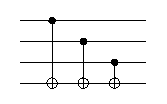
\includegraphics[scale=2]{Figures/circuits/proof1}};   
      \coordinate[below left=7mm and -6mm of c6.west] (l6);
      \coordinate[right=45mm of l6] (r6);
      \pic (cut6) {cut=l6/r6};  
    \end{tikzpicture}
  };
\end{tikzpicture}
\vspace*{140mm}
\caption{Proof of the implementation of multiple non-local CNOT gates that share a common target. The proof uses properties given in Figures~\ref{fig:props}, \ref{fig:sliding} and~\ref{fig:nonlocalCNOTs}. The distributed circuit is similar to the case for share control (Figure~\ref{fig:nonlocalCNOTs}). Both cat-entangler and cat-disentangler slightly differ.}
\label{fig:CNOTtargetProof}
\end{figure}

\section{Finding an efficient distribution}
\label{EfficientDistrib}

In this section we explain how we search for a suitable distribution of the circuit. But first, we establish what we mean by a distributed circuit to be efficient. This is based on what was discussed in \S\ref{DQC_Architecture} to be the bottle-necks of a distributed quantum architecture. A distributed circuit is efficient when there is:

\begin{itemize}
  \item \textit{Minimal amount of quantum communication} between the QPUs, meaning it requires as little number of ebits as possible. In comparison, message passing of classical bits is considered negligible and it is not taken into account.
  \item \textit{Load-balance across the QPUs}, up to a tolerance margin. Our notion of load-balance is that the different QPUs have a similar number of qubits assigned to them. A uniform depth of the local circuits (i.e.\ length of the circuits) would be desirable. However, the distributed circuit depth is inherited from the original circuit, as none of our distribution techniques change the depth in a significant way. Hence, we will not take circuit depth into account, and instead assume that already known methods for depth reduction, such as the one described by~\citet{DepthReduction}, have already been applied on the input circuit, and may be applied again to each QPU's local circuit. As circuit depth is not something we aim to optimise, we consider the cost of local gates negligible.
\end{itemize}

The problem at hand is similar to the  \textit{(\(k,\varepsilon\))-graph partitioning} problem. In it, a graph partition in \(k\) subgraphs has to be found, minimising the number of \textit{cut edges}: edges that have their incident vertices in different subgraphs. Additionally, the resulting partition must satisfy that the number of vertices in each subgraph is less than \((1 \pm \varepsilon)\frac{N}{k}\), where \(N\) is the total number of vertices in the graph. In Table~\ref{tab:matching} we list the correspondences between these two problems.

\begin{table}
\label{tab:matching}
\caption{Correspondence between the graph partitioning problem and the efficient distribution of quantum circuits.}
\centering
\begin{tabular}{|c|c|}
\hline
\textit{Graph partitioning} & \textit{Efficient distribution} \\
\hline
Vertices & Circuit wires \\
Edges & CNOT gates \\
Partitioned graph & Distributed circuit \\
Subgraph & QPU \\
Min. cut edges & Min. non-local gates \\
Uniform subgraph size & Load-balance \\
\hline
\end{tabular}
\end{table}

But there is a caveat. If we use graph partitioning naively, we will not be exploiting the fact that multiple CNOT gates may be implemented using a single ebit. In what follows, we will explain how to make use of \textit{hypergraph} partitioning, instead of simple graph partitioning, to account for this aspect. A more detailed review of the hypergraph partition problem is given in Appendix~\ref{chap:HypPart}, here we summarise the key concepts:

\begin{itemize}
  \item Hypergraphs extend graphs to accommodate edges that may have more than two incident vertices. More formally, a hypergraph is a pair \((V,H)\), where \(V\) is the set of vertices and \(H \subseteq 2^V\) is the collection\footnote{\, We will allow multiple hyperedges connecting the same vertices, in the same way as multigraphs allow multiple edges across any pair of edges.} of hyperedges. Each hyperedge is represented as the subset of vertices from \(V\) it connects. We will not consider any notion of directionality.
  \item Hypergraph partitioning follows the same premise as graph partitioning. The user provides a hypergraph and two parameters \((k,\varepsilon)\), which have the exact same meaning as before. What the problem now attempts to minimise is a metric known as \(\lambda\!-\!1\), which is defined as follows: Given a partition of the hypergraph, the function \(\lambda\colon\, H \to \mathbb{N}\) pairs each hyperedge with the number of different \textit{blocks}\footnote{\, The term \textit{block} is often used to refer to each of the sub-hypergraphs that comprise the hypergraph partition. It is the term we will use throughout this thesis.} its vertices are in. Then, \(\lambda\!-\!1 = \sum_{h \in H} \lambda(h) - 1\) provides a measure of not only how many hyperedges are cut but also how many blocks are they connecting\footnote{\, Simply minimising the number of cut hyperedges is also an often used approach, but it is not as useful for our problem.}.
\end{itemize}

In the following subsections, we explain how hypergraph partitioning can be used to find the best distribution of a circuit. First, we only use the implementation of non-local gates described by~\citet{NonLocalCNOT} reviewed in \S\ref{IntroDistributing}. Later on, we extend the algorithm to include the improvements we have proposed in \S\ref{NonLocalGates}.

\subsection{Vanilla algorithm}
\label{Vanilla}

The key challenge is how to use hyperedges to represent a collection of CNOT gates that, in case of being non-local, they could all be implemented using a single ebit. In this first version of the algorithm, we will group CNOTs together only if they have a common control wire, and there are no other gates in between their connections to that wire. We will create \textit{a single hyperedge} for every such a collection of CNOT gates. The hyperedge's vertices correspond to the controlling wire and each of the different wires the CNOT gates target. Algorithm~\ref{code:buildHypVanilla} builds the hypergraph in that way. It should be noticed that all CNOT gates from the input circuit are represented once and only once in the hypergraph. %This is essential for the well functioning of our approach. 

\begin{algorithm}[caption={Builds the hypergraph of a given circuit. \(H\) may contain multiple hyperedges connecting the same vertices.}, label={code:buildHypVanilla}]
input: circuit
output: (V,H)
begin
  V $\gets$ $\varnothing$
  H $\gets$ $\varnothing$
  hedge $\gets$ $\varnothing$
  foreach wire in circuit do
    V $\gets$ V $+$ {wire}
    H $\gets$ H $+$ {hedge}
    hedge $\gets$ {wire}
    foreach gate in wire do
      if gate == CNOT and $controlOf$(gate) == wire then
        hedge $\gets$ hedge $+$ {$targetOf$(gate)}
      else
        H $\gets$ H $+$ {hedge}
        hedge $\gets$ {wire}
end
\end{algorithm}

%Besides, it may be surprising that our hyperedges do not indicate which of the vertices is the control wire. That information is irrelevant at the partitioning level: each time a hyperedge is cut, we will require an ebit to implement the non-local gates, no matter which QPU the control wire is assigned to. Such information is only relevant when transforming the circuit into its distributed form, which is the next step of our algorithm. 

We then solve the hypergraph partitioning problem (see Appendix~\ref{chap:HypPart}) on the resulting hypergraph. Once an efficient partition of the hypergraph is obtained, we map the partition back to the circuit, distributing it. The resulting partition is interpreted as follows in the circuit:

\begin{itemize}

  \item The way the vertices are assigned in the blocks dictates how the corresponding wires are allocated to the different QPUs. 
  \item Whenever a hyperedge has all of its vertices in the same QPU (i.e.\ it is not cut), all the CNOT gates it represents are implemented locally in that QPU, so no ebit is required. 
  \item If a hyperedge is cut once, some of the wires targeted by the CNOTs will appear in the same QPU as the control wire, so those CNOTs will be implemented locally (Figure~\ref{fig:vanillaCutsA}). The rest of the target wires will be in a different QPU, so the corresponding CNOTs will have to be implemented non-locally, all using the same ebit (Figure~\ref{fig:vanillaCutsB}). 
  \item In the case a hyperedge is cut more than once -- its vertices are split among more than two blocks -- we will proceed in the same manner, but now we will require multiple ebits (Figure~\ref{fig:vanillaCutsC}). As we previously defined, the function \(\lambda\colon H \to \mathbb{N}\) tells us how many blocks a cut hyperedge connects. In order to connect \(\lambda(h)\) blocks, we need at least \(\lambda(h)-1\) block-to-block connections: \(\lambda(h)-1\) ebits. The first halves of all of the ebits is kept by the QPU with the controlling wire, while the rest of the QPUs receive a single half each. This is why the metric we will need our hypergraph partitioner to minimise is \(\lambda-1\).
\end{itemize}

\textbf{TODO} Figure showing the different cases from the paragraph above, a and b. Give both the original circuit with dashed splits, the hypergraph and the black boxed distributed circuit (fig:vanillaCuts)
\begin{figure}
\centering
\begin{tikzpicture}
  \node (distributed) {
    \begin{tikzpicture}
      \node[inner sep=0pt] (circuit) {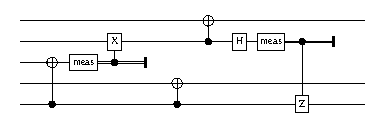
\includegraphics[scale=2]{Figures/circuits/vanillaCuts0}};
      \pic (e1) {ebit=e1/12.67mm/13mm};
      \coordinate[above left=3.6mm and -6mm of circuit.west] (leftPoint);
      \coordinate[above right=3.6mm and -6mm of circuit.east] (rightPoint);
      \pic (cut) {cut=leftPoint/rightPoint};
      \node[above left=11.5mm and -7mm of circuit.west, opacity=0.9] {\footnotesize \(A\)};
      \node[below left=4.5mm and -7mm of circuit.west, opacity=0.9] {\footnotesize \(B\)};
      \node[below left=11.5mm and -7mm of circuit.west, opacity=0.9] {\footnotesize \(C\)};
      \node[right=-3mm of circuit.north west, font=\itshape] (text) {c)};
    \end{tikzpicture}
  };
  \node[above left=-3mm and -70mm of distributed] (template) {
    \begin{tikzpicture}
      \node[inner sep=0pt] (circuit) {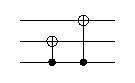
\includegraphics[scale=2]{Figures/circuits/vanillaCutsTemplate}};  
      \coordinate[above left=3.6mm and -6mm of circuit.west] (leftPoint);
      \coordinate[above right=3.6mm and -6mm of circuit.east] (rightPoint);
      \pic (cut) {cut=leftPoint/rightPoint};
      \node[above left=4.5mm and -7mm of circuit.west, opacity=0.9] {\footnotesize \(A\)};
      \node[left=-7mm of circuit.west, opacity=0.9] {\footnotesize \(B\)};
      \node[below left=4.5mm and -7mm of circuit.west, opacity=0.9] {\footnotesize \(C\)};
      \node[right=-3mm of circuit.north west, font=\itshape] (text) {a)};
    \end{tikzpicture}
  };
  \node[above right=-26.5mm and 10mm of template] (hypergraph) {
    \begin{tikzpicture}
      \coordinate (O) at (0,0);
      \coordinate (A) at (90:10mm);
      \coordinate (B) at (210:10mm);
      \coordinate (C) at (330:10mm);
      \draw (O) -- (A);
      \draw (O) -- (B);
      \draw (O) -- (C);
      \node[circle, right=-2.5mm of A, fill=white, inner sep=0pt, minimum size=5mm] {\(A\)};
      \node[circle, right=-2.5mm of B, fill=white, inner sep=0pt, minimum size=5mm] {\(B\)};
      \node[circle, right=-2.5mm of C, fill=white, inner sep=0pt, minimum size=5mm] {\(C\)};
      \coordinate[above left=5.3mm and 9mm of O] (leftPoint);
      \coordinate[above right=5.3mm and 9mm of O] (rightPoint);
      \pic (cut) {cut=leftPoint/rightPoint};
      \node[above left=0mm and 9mm of A, font=\itshape] (text) {b)};
    \end{tikzpicture}
  };
\end{tikzpicture}
\caption{The CNOTs in the circuit \textit{a)} are adjacent at their control wire. Therefore, a single hyperedge is used to represent both in \textit{b)}. The proposed cut makes only one of the CNOTs non-local, which is implemented in \textit{c)} using one ebit.}
\label{fig:vanillaCutsA}
\end{figure}

\begin{figure}
\centering
\begin{tikzpicture}
  \node (distributed) {
    \begin{tikzpicture}
      \node[inner sep=0pt] (circuit) {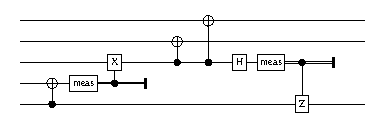
\includegraphics[scale=2]{Figures/circuits/vanillaCuts1}};
      \pic (e1) {ebit=e1/19.75mm/13mm};
      \coordinate[above left=-3.6mm and -6mm of circuit.west] (leftPoint);
      \coordinate[above right=-3.6mm and -6mm of circuit.east] (rightPoint);
      \pic (cut) {cut=leftPoint/rightPoint};
      \node[above left=11.5mm and -7mm of circuit.west, opacity=0.9] {\footnotesize \(A\)};
      \node[above left=4.5mm and -7mm of circuit.west, opacity=0.9] {\footnotesize \(B\)};
      \node[below left=11.5mm and -7mm of circuit.west, opacity=0.9] {\footnotesize \(C\)};
      \node[right=-3mm of circuit.north west, font=\itshape] (text) {c)};
    \end{tikzpicture}
  };
  \node[above left=-3mm and -70mm of distributed] (template) {
    \begin{tikzpicture}
      \node[inner sep=0pt] (circuit) {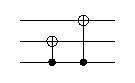
\includegraphics[scale=2]{Figures/circuits/vanillaCutsTemplate}};  
      \coordinate[below left=3.6mm and -6mm of circuit.west] (leftPoint);
      \coordinate[below right=3.6mm and -6mm of circuit.east] (rightPoint);
      \pic (cut) {cut=leftPoint/rightPoint};
      \node[above left=4.5mm and -7mm of circuit.west, opacity=0.9] {\footnotesize \(A\)};
      \node[left=-7mm of circuit.west, opacity=0.9] {\footnotesize \(B\)};
      \node[below left=4.5mm and -7mm of circuit.west, opacity=0.9] {\footnotesize \(C\)};
      \node[right=-3mm of circuit.north west, font=\itshape] (text) {a)};
    \end{tikzpicture}
  };
  \node[above right=-30mm and 10mm of template] (hypergraph) {
    \begin{tikzpicture}
      \coordinate (O) at (0,0);
      \coordinate (A) at (90:10mm);
      \coordinate (B) at (210:10mm);
      \coordinate (C) at (330:10mm);
      \draw (O) -- (A);
      \draw (O) -- (B);
      \draw (O) -- (C);
      \node[circle, right=-2.5mm of A, fill=white, inner sep=0pt, minimum size=5mm] {\(A\)};
      \node[circle, right=-2.5mm of B, fill=white, inner sep=0pt, minimum size=5mm] {\(B\)};
      \node[circle, right=-2.5mm of C, fill=white, inner sep=0pt, minimum size=5mm] {\(C\)};
      \coordinate (leftPoint) at (270:10.5mm);
      \coordinate (rightPoint) at (30:10.5mm);
      \pic (cut) {cut=leftPoint/rightPoint};
      \node[above left=0mm and 9mm of A, font=\itshape] (text) {b)};
    \end{tikzpicture}
  };
\end{tikzpicture}
\caption{Same as in Figure~\ref{fig:vanillaCutsA}, but now the cut makes both CNOTs non-local. Still, only one ebit is required, as implied by the hypergraph \textit{b)}. When CNOTs share their control wire, an ebit is required iff any of the target wires is in a different QPU than the control wire's QPU.}
\label{fig:vanillaCutsB}
\end{figure}

\begin{figure}
\hspace*{0mm}
\begin{tikzpicture}
  \node (template) {
    \begin{tikzpicture}
      \node[inner sep=0pt] (circuit) {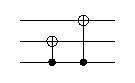
\includegraphics[scale=2]{Figures/circuits/vanillaCutsTemplate}};  
      \coordinate[below left=3.6mm and -6mm of circuit.west] (leftPoint1);
      \coordinate[below right=3.6mm and -6mm of circuit.east] (rightPoint1);
      \pic (cut1) {cut=leftPoint1/rightPoint1};
      \coordinate[above left=3.6mm and -6mm of circuit.west] (leftPoint2);
      \coordinate[above right=3.6mm and -6mm of circuit.east] (rightPoint2);
      \pic (cut2) {cut=leftPoint2/rightPoint2};
      \node[above left=4.5mm and -7mm of circuit.west, opacity=0.9] {\footnotesize \(A\)};
      \node[left=-7mm of circuit.west, opacity=0.9] {\footnotesize \(B\)};
      \node[below left=4.5mm and -7mm of circuit.west, opacity=0.9] {\footnotesize \(C\)};
      \node[right=-3mm of circuit.north west, font=\itshape] (text) {a)};
    \end{tikzpicture}
  };
  \node[above right=-28mm and 10mm of template] (hypergraph) {
    \begin{tikzpicture}
      \coordinate (O) at (0,0);
      \coordinate (A) at (90:10mm);
      \coordinate (B) at (210:10mm);
      \coordinate (C) at (330:10mm);
      \draw (O) -- (A);
      \draw (O) -- (B);
      \draw (O) -- (C);
      \node[circle, right=-2.5mm of A, fill=white, inner sep=0pt, minimum size=5mm] {\(A\)};
      \node[circle, right=-2.5mm of B, fill=white, inner sep=0pt, minimum size=5mm] {\(B\)};
      \node[circle, right=-2.5mm of C, fill=white, inner sep=0pt, minimum size=5mm] {\(C\)};
      \coordinate[above left=5.3mm and 9mm of O] (leftPoint);
      \coordinate[above right=5.3mm and 9mm of O] (rightPoint);
      \pic (cut) {cut=leftPoint/rightPoint};
      \coordinate (leftPoint2) at (270:10.5mm);
      \coordinate (rightPoint2) at (30:10.5mm);
      \pic (cut2) {cut=leftPoint2/rightPoint2};
      \coordinate (extraPoint) at (30:16mm);
      \pic (cut3) {cut=rightPoint2/extraPoint};
      \node[above left=0mm and 9mm of A, font=\itshape] (text) {b)};
    \end{tikzpicture}
  };
  \node[below right=2mm and -73mm of template] (distributed) {
    \begin{tikzpicture}[transform canvas={scale=0.65}]
      \node[inner sep=0pt] (circuit) {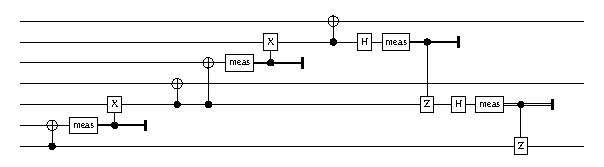
\includegraphics[scale=2]{Figures/circuits/vanillaCuts2}};
      \pic (e1) {ebit=e1/12.67mm/13mm};
      \pic (e2) {ebit=e2/33.84mm/13mm};
      \coordinate[above left=10.6mm and -6mm of circuit.west] (leftPoint);
      \coordinate[above right=10.6mm and -6mm of circuit.east] (rightPoint);
      \pic (cut) {cut=leftPoint/rightPoint};
      \coordinate[below left=10.6mm and -6mm of circuit.west] (leftPoint2);
      \coordinate[below right=10.6mm and -6mm of circuit.east] (rightPoint2);
      \pic (cut2) {cut=leftPoint2/rightPoint2};
      \node[above left=18.5mm and -7mm of circuit.west, opacity=0.9] {\footnotesize \(A\)};
      \node[left=-7mm of circuit.west, opacity=0.9] {\footnotesize \(B\)};
      \node[below left=18.5mm and -7mm of circuit.west, opacity=0.9] {\footnotesize \(C\)};
    \end{tikzpicture}
  };
  \node[right=-3mm of distributed.north west, font=\itshape] (text) {c)};
\end{tikzpicture}
\vspace*{38mm}
\caption{Same as in Figure~\ref{fig:vanillaCutsA}, but now there are two cuts, distributing the circuit across three QPUs.}
\label{fig:vanillaCutsC}
\end{figure}

Following this intepretation of the hypergraph partition, we transform the original circuit to obtain its distributed version. To do so, for each cut hyperedge \(h\), we insert \(\lambda(h)-1\) cat-entanglers just before the group of CNOT gates it represents; and \(\lambda(h)-1\) cat-disentanglers right after them. Then, each of the CNOTs that have to be implemented non-locally are modified so their control wire is the corresponding QPU's local ebit half, while the target is unchanged.

%Notice that if procedure from Algorithm~\ref{code:distribution} is applied carelessly, the ordering of the gates could be altered, as a CNOT gate could be inserted before the previous gates on the target wire have been added. Some bookmarking must be kept to prevent this, but the details are straight-forward.

\begin{comment}
\begin{algorithm}[caption={Algorithm for distributing a circuit using an assignment \(qpuOf \colon \mathbb{N} \to \mathbb{N}\) which indicates the QPU number of the given wire},label={code:distribution}]
input: circuit, $qpuOf$
output: distributed
begin
  distributed $\gets$ $emptyCircuit$
  foreach wire in circuit do
    thisQPU = $qpuOf$(wire)
    activeConnections $\gets$ $\varnothing$
    foreach gate in wire do
      if gate == CNOT and $controlOf$(gate) == wire then
        targetQPU = $qpuOf$($targetOf$(gate))
        if targetQPU == thisQPU then
          distributed.$addCNOTAt$(wire,target)
        else
          ebit $\gets$ activeConnections.$at$(targetQPU)
          if ebit == null then
            ebit $\gets$ $distillEbit$(thisQPU, targetQPU)
            distributed.$addCatEntangler$(ebit, wire)
            activeConnections.$at$(targetQPU) $\gets$ ebit
          distributed.$addCNOTAt$(ebit,$targetOf$(gate))
      else
        distributed.$addGateAt$(gate,wire)
end
\end{algorithm}
\end{comment}


\textbf{TODO}: A figure showing a simple circuit, its hypergraph and its distributed circuit (with cat-(dis)entangler as a box). It'd be great if the example on these three subsections was the same (fig:distribProcess)

A simple example of the distribution process is shown in Figure~\ref{fig:distribProcess}. The resulting circuit is a distributed version of the original one, that is efficient in the sense described in the beginning of this section. Each of the QPUs can be set to implement its own local circuit, distilling ebits and using them along classical communication whenever indicated.


\subsection{Bringing CNOT gates together}
\label{pullCNOTs}

In \S\ref{NonLocalGates} we have shown that any 1-qubit gate in the Clifford+T set acting on the control wire of a CNOT gate, with the exception of the H gate, can commute with the CNOT up to some byproduct. Here we use this fact, applying some preprocessing on the input circuit that brings together nearby CNOT gates, allowing us to implement more non-local CNOT gates using a single ebit. Figure~\ref{fig:pulledCNOTexample} gives an example of how these transformations -- listed in Figures \textbf{TODO} -- can lead to a more efficient distribution of the circuit.

\textbf{TODO} Figure with (hopefully) the same circuit as the previous figure, its version after CNOTpulling and its hypergraph partition, which should have less lambda-1 (fig:pulledCNOTexample)

The preprocessing procedure is fairly straight-forward: Exploring the circuit from left to right, whever a CNOT gate is found, use the transformations listed in Figure~\ref{fig:pullRules} to move it as early in the circuit as possible. The procedure introduces some additional \(X\) gates. Fortunately, \(X\) is its own inverse (i.e.\ \(XX = I\)) and every 1-qubit gate in Clifford+T can be interchanged with \(X\) in a simple way (as shown in Figure~\ref{fig:props}). Hence, we should not expect a significant increase in the depth of the circuit, as most byproduct gates will cancel each other out.

So far we have been talking about standard 1-qubit gates, but in practical circuits we are likely to find 1-qubit gates that are \textit{classically-controlled}, meaning that a classical signal (a bit, either \(0\) or \(1\)) decides whether the gate is applied or not. These are no issue for the distribution of the circuit, as this classical control may only require classical communication between QPUs. Concerning the preprocessing we just described, classically-controlled 1-qubit gates can commute with CNOT under the exact same circumstances as their uncontrolled version. The only difference is that, whenever a byproduct gate is created, we must make sure it is controlled by the same classical signal that controlled the original gate, as shown in Figure~\ref{fig:classicalControl}.

\textbf{TODO} Figure with an X gate classically controlled before the control of a CNOT. Then the resulting circuit after exchanging them (fig:classicalControl)

The same procedure can be used to commute 1-qubit gates across the target wire of the CNOT gates, although in this case, apart from \(H\), \(S\) and \(T\) gates can not commute either. This additional preprocessing would have no effect at all on the vanilla version of the algorithm, but it will be beneficial after we apply our next extension, which requires CNOT gates to be adjacent on the target wire.


\subsection{Adding the common-target method}
\label{BothEnds}

In \S\ref{NonLocalGates} we showed that the trick for implementing multiple CNOT gates using a single ebit also works if they share a common target wire (instead of the control wire). This makes our optimisation problem more intricate: Before, for each CNOT gate we only had two options, either to make it local or non-local -- whether to cut the hyperedges or not. But now, when the CNOTs are to be implemented non-locally, we can choose to implement them using the common-control or common-target method. In order to represent this choice in our hypergraphs, we will use two different kinds of hyperedges, whether what their CNOTs have in common is the control or the target. Figure~\ref{fig:BothEndsSimple} shows a simple circuit where neither of the options is a priori better. 

\textbf{TODO}: Figure where with 3 CNOTs we show that depending on how they are grouped together, we may gain something or not, which ultimately depends on how the hypergraph is split. Include both hypergraphs (fig:BothEndsSimple) Caption: The hypergraph of the circuit built as in Algorithm~\ref{code:buildHypVanilla} uses the common control of gates \(\alpha\) and \(\beta\), while the other one is built similarly, but on common target. Different line format for the hyperedges whether control or target.

Now, imagine the circuit from Figure~\ref{fig:BothEndsSimple} to be a fragment of a larger one. Then, it may happen that the rest of the circuit makes the most efficient distribution allocates wires \(A\) and \(B\) in one QPU and wire \(C\) in another. As shown in Figure~\ref{fig:BothEndsChallenge}, in this particular case using the common-target method saves us one ebit. Conversely, if \(A\) were the wire on a separate QPU and \(B,C\) were together, using the common-control method would be best. The conclusion is that the choice of control or target hyperedges on a particular fragment of the circuit is dependent on the overall partitioning. 

Therefore, it would be best to build the hypergraph in such a way that the decision of using control or target hyperedges is not done a priori, but by the hypergraph partitioner itself. A naive approach, also shown in Figure~\ref{fig:BothEndsChallenge}, would be to include all of the hyperedges, both of control and target type, in the same hypergraph. But then either partitioning of the hypergraph cuts three hyperedges, so the hypergraph partitioner sees no difference between the two options, preventing it from taking into account this subtlety when optimising.

\textbf{TODO}: Figure of hypergraphs from prev Fig; with control hyps, target hyps, naively. The dashed lines represent two hypothetical ways of partitioning the hypergraph. Different line format for the hyperedges whether control or target (fig:BothEndsChallenge)

We propose to build the hypergraph as in Algorithm~\ref{code:buildHypBothEnds}. This hypergraph requires an additional vertex per CNOT in the circuit, and the block where the hypergraph partitioner decides to include that vertex in dictates whether the CNOT is implemented as a control or target hyperedge. Figure~\ref{fig:BothEndsProcess} shows how the hypergraph is built step by step for our running example. 

\begin{algorithm}[caption={Builds the hypergraph of a given circuit, without choosing whether CNOT gates are implemented through common control or common target.}, label={code:buildHypBothEnds}]
input: circuit
output: (V,H)
begin
  V $\gets$ $\varnothing$
  H $\gets$ $\varnothing$
  hedge $\gets$ $\varnothing$
  foreach wire in circuit do
    V $\gets$ V $+$ {wire}
    H $\gets$ H $+$ {hedge}
    hedge $\gets$ {wire}
    hType $\gets$ $unknown$
    foreach gate in wire do
      if gate == CNOT then
        if $controlOf$(gate) == wire then
          if hType == $target$ then
            H $\gets$ H $+$ {hedge}
            hedge $\gets$ {wire}
          hType $\gets$ $control$
        if $targetOf$(gate) == wire then
          if hType == $control$ then
            H $\gets$ H $+$ {hedge}
            hedge $\gets$ {wire}  
          hType $\gets$ $target$
        hedge $\gets$ hedge $+$ {$labelOf$(gate)}
      else
        H $\gets$ H $+$ {hedge}
        hType $\gets$ $unknown$
        hedge $\gets$ {wire}
end
\end{algorithm}

\textbf{TODO}: Figure where the hypergraph for the three CNOTs example is built step by step (as in the Algorithm above) (fig:BothEndsProcess)

The hypergraph built by Algorithm~\ref{code:buildHypBothEnds} has one caveat: When discussing load-balancing in \S\ref{EfficientDistrib}, we explained that we were interested in allocating a uniform number of wires to each QPU. Previously, the hypergraph partitioner took care of this, as it tried to assign a uniform number of vertices to each block. But now, the hypergraph partitioner has no way of distinguishing between `wire' vertices and `CNOT' vertices, the latter being an artificial gadget that should not count towards load-balancing. The solution is simple, instead of the standard hypergraph partition problem, we apply a version of it where vertices can have a weight assigned (see Appendix~\ref{chap:HypPart}). Then, each wire-vertex is given weight \(1\), and each CNOT-vertex is given weight \(0\), effectively ignoring them for the load-balancing aspect.

We now explain how the hypergraph partition determines the distribution of the circuit:

\begin{itemize}
  \item As in the vanilla version of the algorithm, the way wire-vertices are assigned to blocks determines how wires are allocated to QPUs.
  \item In the vanilla version, if a hyperedge was cut in \(\lambda(h)\) blocks, we needed \(\lambda(h)-1\) ebits. The first halves of all of them were kept by the QPU with the control wire, while the rest of the QPUs received one ebit half each. Now, the exact same thing will happen for cuts on hyperedges of the control type, while in the case of target hyperedges, it is the QPU holding the target wire the one that keeps the one half of all the ebits. 
  \item The block where a CNOT-vertex is assigned dictates in which QPU the CNOT operation itself is carried out. As we discussed in \S\ref{NonLocalGates}, if the non-local CNOT is implemented using the common-control method, the CNOT is applied in the target QPU, and vice versa. Hence, the block where the CNOT-vertex is assigned indicates the method that should be used to implement it. 
\end{itemize}

An example is shown in Figure~\ref{fig:modes}. Notice that the ebit required to implement each of the non-local CNOTs is guaranteed to exist as, by construction (Algorithm~\ref{code:buildHypBothEnds}), each CNOT-vertex is always connected to exactly two wire-vertices, corresponding to its control and target wires. Whenever these three vertices are not assigned to the same QPUs, a hyperedge will be cut, and the required ebit will be generated.

\begin{mdframed}[backgroundcolor=gray!20,leftmargin=20pt,rightmargin=20pt, innerbottommargin=10pt] 
\small
\textbf{Remark:} It is easy to check that the distributed circuit we obtain using the vanilla algorithm (from \S\ref{Vanilla}) is the same as the one obtained by this approach, restricting it so either:
\begin{enumerate}
  \renewcommand{\theenumi}{\alph{enumi})}
  \item The common-target trick is never used.
  \item CNOT gates are always executed in their target QPU.
  \item Our hypergraph partitioner never cuts target hyperedges.
\end{enumerate}
\end{mdframed}

Under this interpretation it is apparent that the problem of efficiently distributing a circuit using the common-control and common-target methods, and the problem of partitioning the hypergraph built by Algorithm~\ref{code:buildHypBothEnds}, are indeed the same. All the relevant information from the circuit -- all the possible choices of how to implement each an every CNOT in the circuit -- is encoded in the hypergraph, while each aspect of the hypergraph partition can be mapped back to the circuit.

It is interesting to discuss the particular case in Figure~\ref{fig:farCNOT}. Here, a CNOT gate that must be applied non-locally between QPU \(1\) and QPU \(2\), ends up having its local fragment -- the CNOT-vertex, and thus the CNOT gate itself --  in neither of them, but in a distant QPU \(3\). This happens whenever QPU \(1\) and QPU \(2\) do not share the necessary ebit, but they are both sharing a suitable ebit with QPU \(3\). Intuitively, it can be seen as passing a message through a middle-man; sometimes, using communication through an already available middle-man is better than putting up a full blown connection just for a single message. The hypergraph partitioner acting on the hypergraph built by Algorithm~\ref{code:buildHypBothEnds} will automatically use this strategy whenever it reduces the number of ebits required. Notice, however, that this trick only allows to implement a single CNOT with both target and control wires in some particular QPUs. When the CNOT shares one of its wires with multiple CNOTs, it will often be best to use the common-control or common-target method to implement all of them together. This trick will be useful whenever there are stray CNOT gates that can not be efficiently grouped with other CNOTs.

\textbf{TODO}: The case where a non-local CNOT is actually applied in neither of the QPUs at its ends, the circuit is the 3CNOT example from BothEndsSimple, split in three (fig:farCNOT)

In any case, some criticism must be considered here: if we put no constraint on the exploitation of `middle-men' QPUs, it may happen that communication across many of the QPUs all use the same middle-man QPU to deliver their messages, potentially creating a bottle neck. We see two ways around this:

\begin{enumerate}
\item Accept that some circuits will naturally be prone to such a centralised communication network, where a few QPUs must be prepared to carry most of the communication work. This does happen in classical networking too, and sometimes the best option is a centralised system. As far as the hardware is designed with these needs in mind, centralisation may not be a bottle neck, but even an advantage. 

\item In case really wish to have a decentralised network, you will need to find a way to ensure the hypergraph partition you get has some kind of load-balancing on communication. Fortunately, there is a simple way of load-balancing the usage of ebits: instead of giving CNOT vertices weight \(0\) as we previously discussed, we may give them some weight \(\mu > 0\) that indicates how relevant communication load-balancing is in comparison to the uniformity of wire allocation across QPUs. Even better, we could use a custom version of the hypergraph partitioning problem where we provide three parameters instead of two, \(k,\varepsilon,\eta\), where now \(\varepsilon\) acts as the tolerance for imbalance of wire-vertices, while \(\eta\) is a separate tolerance for imbalance of CNOT-vertices, both tolerances being enforced in any partition.
\end{enumerate}


Across the figures of this subsection we have drawn differently hyperedges that group CNOTs with common-control or common-target. However, it should be noticed that the hypergraph partitioner does not use this information at any point. This distinction is made for explanation purposes, and it is only relevant when building the distributed version of the circuit. The procedure for distributing the circuit following a given hypergraph partition is very similar to that in the vanilla version of the algorithm (see \S\ref{Vanilla}). The only difference is that cat-entanglers and cat-disentanglers are slightly different whether the CNOT is implemented through common-control or common-target (see Figure~\ref{fig:CNOTtargetProof}).

As a wrap up of this section, in Figure~\ref{fig:modes} we show the same circuit being distributed in four different ways: with or without the extension from \S\ref{pullCNOTs} and with or without the extension from \S\ref{BothEnds}. This provides a simple example where both extensions are shown to reduce the number of ebits required to distribute a circuit.

\textbf{TODO} Figure example `interesting' with different modes (fig:modes)

\section{Interchanging CNOT gates}

CNOT gates trivially commute when they are applied to different wires. When one of the wires is in common, if it has the same role (control or target) for both CNOTs, we can take advantage of it and implement them using a single ebit, as we just described. If both wires are in common and have the same role, the CNOTs cancel each other. But what happens if two CNOTs act on the same wire with different roles? In that case, we can still interchange the gates as in Figure~\textbf{TODO}, but that creates an additional CNOT per interchange.

\textbf{TODO}: Interchange challenge, only the two circuits with the dashed split and their respective hypergraphs (fig:interchangeChallenge)

It may seem like preprocessing the circuit so it has the minimum possible number of CNOT gates would always be the best option for partitioning. However, this is not always true, as shown in Figure~\ref{fig:interchangeChallenge}. In some cases interchanging CNOTs may unlock a more efficient partitioning of the circuit, regardless of it adding more CNOTs. In other cases, it will have no benefit, and add an extra CNOT to take into account when partitioning. This compromise prevents us from knowing a priori the best choice. Providing the hypergraph partitioner with the flexibility of deciding either to interchange a particular pair of CNOTs or not -- in the same spirit we did in \S\ref{BothEnds} -- would be the best solution. However, encoding such a choice in a hypergraph partitioning problem is very difficult, due to the following reasons:

\begin{enumerate}
  \item \textit{The way CNOT gates are ordered in the circuit is important}: This is something we omit in the hypergraph built by Algorithm~\ref{code:buildHypBothEnds}; looking at the final hypergraph in Figure~\ref{fig:BothEndsProcess}, we can not tell whether \(\alpha\) goes before or after \(\beta\). This information is key when interchanging, as it will determine which are the new neighbours of the interchanged CNOTs. This could potentially be accounted for by imposing that any hyperedge is an ordered list of vertices\footnote{\, For instance, the first vertex corresponding to a circuit wire and the rest, corresponding to the different CNOT gates, ordered as in the circuit.}. However, the standard hypergraph partitioning problem does not take into account such ordering, so we would need to define a custom hypergraph partitioning problem where this information is somehow taken into account.

  \item \textit{Interchanging CNOT gates adds new CNOTs}: This problem is substantially different from the problem in \S\ref{BothEnds}, where the count of CNOTs remained the same, and thus the only degree of freedom was whether each CNOT was implemented as control or as target hyperedge. The essence of our solution in \S\ref{BothEnds} is to represent all of the options in the hypergraph. However, if were to interchange a pair of CNOTs, new choices would become available: Is it worth to interchange the CNOTs again with their new neighbours? Should the byproduct CNOT be itself interchanged further? Although the number of options to take into account is finite, it is considerably larger. And what is worse, each choice would not be independent from the rest -- as some interchanges are only available if others have been done before -- so the structure of the hypergraph would likely be quite complex to accommodate this aspect.
\end{enumerate}

Instead of encoding this choice within the hypergraph partioning problem, another option is to apply some postprocessing once the circuit has been partitioned. This postprocessing would exhaustively apply the transformations in Figures~\textbf{TODO} to each pair of potentially interchangeable CNOTs, keeping those transformations that reduced the ebit count. 

\textbf{TODO} Is this a greedy algorithm? (most probably, a greedy algorithm won't be optimal) Should I give more details on the strategy? Am I implementing this too?

\section{An upper bound}

\textbf{TODO}: Finally, for the sake of comparison, we will use some theoretical results on quantum circuit decomposition, in order to estimate an upper bound of the number of ebits needed to distribute any quantum process on \(N\) qubits.

\textbf{TODO}: Discuss structured vs unstructured as the reason why we expect our algorithm to perform better.
